\documentclass[12pt,a4paper,margin=2cm]{book}





% The "ulem" package enables the use of ``strike-out'': e.g. \sout{Text to be struck}
\usepackage{ulem}

% The "makeidx" package enables the creation of an index for the book
\usepackage{makeidx}

% The "graphicx" package allows image widths to be specified: e.g. \includegraphics[width=4in]{junk.eps} 
\usepackage[dvips]{graphicx} 

% The "array" package allows manipulation of table row height using the "extrarowheight" setlength option
\usepackage{array}
\usepackage{amsmath}

\usepackage{xcolor}

% The "listings" package enables programming source code to be formatted in an attractive way
\usepackage{listings}
\usepackage{makecell} % gjør det mulig å gjøre linjebytte i en enkelt celle \makecell{}
% The "hyperref" package enables hyperlinks in the dvi, PostScript, and PDF output files
% for easier navigation.  This includes hyperlinked index and TOC entries!
\usepackage[
	pdftitle = "{Automatiseringssystemer For Gand VGS}",
    pdfauthor = "{Fred-Olav Mosdal}",
%    dvips = false,
%    ps2pdf = false,
%    pdftex,
    colorlinks = true,
    breaklinks= true,
    hyperindex = true
]{hyperref}

% Define "pseudocode" as a language recognized by the "listings" package:
\lstdefinelanguage{pseudocode}
{morekeywords={DECLARE,BEGIN,END,LOOP,ENDLOOP,SET,IF,THEN,CALL,RETURN,ELSEIF,ELSE,ENDIF,PRINT,OUTPUT,AND,OR},
 morecomment=[l]{//}
}

\lstloadlanguages{pseudocode,[ANSI]C}

% Set some of the environment variables for the "listings" package to format source code:
%\lstset{frame=single,language=pseudocode,keywordstyle=\color{blue}\bfseries,commentstyle=\color{red}\itshape}
\lstset{frame=single,keywordstyle=\color{blue}\bfseries,commentstyle=\color{red}\itshape}

\setlength{\parskip}{1em}
\setlength{\parindent}{0em}


% These commands set widths of text, and margins:
\setlength{\textwidth}{16cm}
\setlength{\evensidemargin}{0cm}
\setlength{\oddsidemargin}{0cm}
\setlength{\extrarowheight}{3pt} % adds extra space to the top of each LaTeX ("tabular") table row to make superscripted math expressions look better

% This command prompts the compilation of an index
\makeindex









% This begins the document:
\begin{document}


% Set some of the environment variables for the "listings" package to format source code:
%\lstset{frame=single,language=pseudocode,keywordstyle=\color{blue}\bfseries,commentstyle=\color{red}\itshape}








%% Cover %%







%% Copyright page %%


%
%
%
%
%
%
%%% Table of contents %%
%
\tableofcontents  
\cleardoublepage
\pagenumbering{arabic}








%% Preface %%

\vfil \eject


%%%%%%%%%%%%%%%%%%%%%%%%%%%%%%%%%%%%%%%%%%%%%%%%%%%%
%% Begin book chapters, sections, and subsections %%
%%%%%%%%%%%%%%%%%%%%%%%%%%%%%%%%%%%%%%%%%%%%%%%%%%%%

%\input PrefaceByTony.tex
%
%\input Calculus.tex 
%\input Physics.tex
%\input Chemistry.tex
%\input ACelectricity.tex
%\input IntroductionToIndustrialInstrumentation.tex
%\input InstrumentationDocuments.tex
%\input InstrumentConnections.tex
%\input DiscreteProcessMeasurement.tex
%\input DiscreteControlElements.tex
%\input RelayControlSystems.tex
%\input PLC.tex
%\input PLS.tex
%\input AnalogElectronicInstrumentation.tex
%\input PneumaticInstrumentation.tex
%\input DigitalDataAcquisitionAndNetworks.tex
%\input FoundationFieldbusInstrumentation.tex
%\input WirelessInstrumentation.tex
%\input InstrumentCalibration.tex
%\input ContinuousPressureMeasurement.tex
%\input ContinuousLevelMeasurement.tex
%\input ContinuousTemperatureMeasurement.tex
%\input ContinuousFluidFlowMeasurement.tex
%\input ContinuousAnalyticalMeasurement.tex
%\input MachineVibrationMeasurement.tex
%\input ElectricPowerMeasurementAndControl.tex
%\input SignalCharacterization.tex
%\input InferentialMeasurement.tex  %Dead Chapter
%\input ControlValves.tex
%\input VariableSpeedMotorControls.tex
\input ClosedLoopControl.tex
%\input ProcessDynamicsAndPIDControllerTuning.tex
%\input BasicProcessControlStrategies.tex
%\input ProcessSafetyAndInstrumentation.tex
%\input InstrumentationCyberSecurity.tex
%\input ProblemSolvingAndDiagnosticStrategies.tex
%\input FlipBookAnimations.tex
%\input DoctorStrangeflow.tex
%\input DisassemblyOfaSlidingStemControlValve.tex
%\input HowToUseThisBook.tex
%\input Contributors.tex
%\input CreativeCommonsAttributionLicense.tex



%%%%%%%%%%%%%%%%%%%%%%%%%%%%%%%%%%%%%%%%%%%%%%%%%%%%

%%%%%%%%%%%%%%%%%%%%%%
%% Begin book index %%
%%%%%%%%%%%%%%%%%%%%%%

\printindex



%% The end! %%
\end{document}
\end{book}


